\documentclass[a4paper,12pt]{report}
\usepackage{graphicx}
\graphicspath{{picaa/}}
\usepackage{listings}
\usepackage{amsmath}
\usepackage[T2A]{fontenc}
\usepackage[utf8]{inputenc}
\usepackage[english,russian]{babel}
\usepackage{pgfplots} 
\usepackage{indentfirst}
\parindent=1cm

\usepackage{geometry}
\geometry{left=2cm}
\geometry{right=1.5cm}
\geometry{top=1cm}
\geometry{bottom=2cm}
\lstset{language = Python,
keywordstyle = \color{orange},
stringstyle = \color{green},
commentstyle = \color{red},
columns = fullflexible,
captionpos = t
}
\lstset{
	literate={а}{{\selectfont\char224}}1
	{б}{{\selectfont\char225}}1
	{в}{{\selectfont\char226}}1
	{г}{{\selectfont\char227}}1
	{д}{{\selectfont\char228}}1
	{е}{{\selectfont\char229}}1
	{ё}{{\"e}}1
	{ж}{{\selectfont\char230}}1
	{з}{{\selectfont\char231}}1
	{и}{{\selectfont\char232}}1
	{й}{{\selectfont\char233}}1
	{к}{{\selectfont\char234}}1
	{л}{{\selectfont\char235}}1
	{м}{{\selectfont\char236}}1
	{н}{{\selectfont\char237}}1
	{о}{{\selectfont\char238}}1
	{п}{{\selectfont\char239}}1
	{р}{{\selectfont\char240}}1
	{с}{{\selectfont\char241}}1
	{т}{{\selectfont\char242}}1
	{у}{{\selectfont\char243}}1
	{ф}{{\selectfont\char244}}1
	{х}{{\selectfont\char245}}1
	{ц}{{\selectfont\char246}}1
	{ч}{{\selectfont\char247}}1
	{ш}{{\selectfont\char248}}1
	{щ}{{\selectfont\char249}}1
	{ъ}{{\selectfont\char250}}1
	{ы}{{\selectfont\char251}}1
	{ь}{{\selectfont\char252}}1
	{э}{{\selectfont\char253}}1
	{ю}{{\selectfont\char254}}1
	{я}{{\selectfont\char255}}1
	{А}{{\selectfont\char192}}1
	{Б}{{\selectfont\char193}}1
	{В}{{\selectfont\char194}}1
	{Г}{{\selectfont\char195}}1
	{Д}{{\selectfont\char196}}1
	{Е}{{\selectfont\char197}}1
	{Ё}{{\"E}}1
	{Ж}{{\selectfont\char198}}1
	{З}{{\selectfont\char199}}1
	{И}{{\selectfont\char200}}1
	{Й}{{\selectfont\char201}}1
	{К}{{\selectfont\char202}}1
	{Л}{{\selectfont\char203}}1
	{М}{{\selectfont\char204}}1
	{Н}{{\selectfont\char205}}1
	{О}{{\selectfont\char206}}1
	{П}{{\selectfont\char207}}1
	{Р}{{\selectfont\char208}}1
	{С}{{\selectfont\char209}}1
	{Т}{{\selectfont\char210}}1
	{У}{{\selectfont\char211}}1
	{Ф}{{\selectfont\char212}}1
	{Х}{{\selectfont\char213}}1
	{Ц}{{\selectfont\char214}}1
	{Ч}{{\selectfont\char215}}1
	{Ш}{{\selectfont\char216}}1
	{Щ}{{\selectfont\char217}}1
	{Ъ}{{\selectfont\char218}}1
	{Ы}{{\selectfont\char219}}1
	{Ь}{{\selectfont\char220}}1
	{Э}{{\selectfont\char221}}1
	{Ю}{{\selectfont\char222}}1
	{Я}{{\selectfont\char223}}1
}

\begin{document}

    \begin{titlepage}

        \begin{center}
            \large
            \textbf{Государственное образовательное учреждение высшего профессионального образования\\
            “Московский государственный технический университет имени Н.Э.Баумана”\\}
            
\includegraphics{bmstu-logo.png}
			\vspace{1cm}
            
            \textsc{Дисциплина: Анализ алгоритмов}
            \vspace{0.5cm}
                
            \textsc{Рубежный контроль №2}
            \vspace{1cm}
            
            {\LARGE \textbf{Нахождение подстроки в строке с помощью регулярных выражений и конечного автомата}}
            \vspace{3cm}
                    
            \begin{flushright}
            	Студент группы ИУ7-55Б,\\   
            	Руднев К. К.,\\
            	\vspace{0.5cm}
            	Преподаватель,\\
            	Волкова Л. Л.,\\
            	Строганов Ю. В.
            	
            \end{flushright}
            \vfill
            
            2019 г.
            
        \end{center}

    \end{titlepage}

	\setcounter{page}{2}
    \newpage

    \begin{center}
        \textbf{1 Аналитическая часть}
    \end{center}
        \label{sec:analitic_part}

        	В рамках раздела будет дано аналитическое описание регулярных выражений и конечного автомата.

	\begin{center}
        \textbf{1.1 Описание алгоритмов}
    \end{center}

		\begin{center}
			\textbf{1.1.1 Регулярные выражения}
		\end{center}
	
	       Регулярные выражения — формальный язык поиска и осуществления манипуляций с подстроками в тексте, основанный на использовании метасимволов. 
	       Для поиска используется строка-образец, состоящая из символов и метасимволов и задающая правило поиска.
	       Для манипуляций с текстом дополнительно задаётся строка замены, которая также может содержать в себе специальные символы.
	       
		\begin{center}
			\textbf{1.1.2 Конечный автомат}
	    \end{center}
   
		   Конечный автомат можно охарактеризовать множеством состояний (вершин) и переходов (дуг, соединяющие вершины). 
		   Среди состояний есть два специальных - состояние начала и конца. 
		   Если строка читается данным автоматом, то после прохода по строке, автомат должен оказаться в одном из заключительных состояний. 
		   На этом основывается алгоритм поиска подстроки в строке с помощью конечного автомата.

    \newpage

    \begin{center}
        \textbf{2 Конструкторская часть}
    \end{center}
        \label{sec:construct_part}

			В дальнейшем на рисунке \ref{ris:automat} будет представлена схема разработанного автомата.

	\begin{center}
        \textbf{2.1 Разработка алгоритмов}
    \end{center}

		\begin{figure}[h!]
			\center{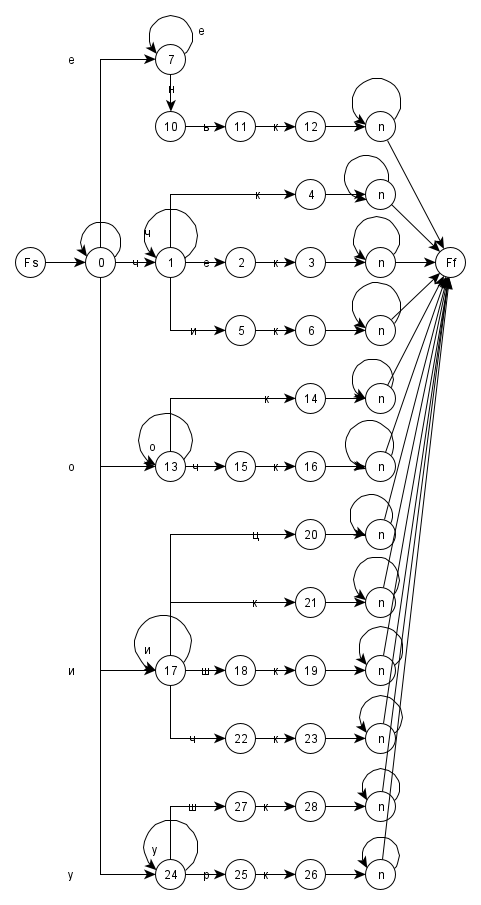
\includegraphics[width=0.65\linewidth]{automat1.png}}
			\caption{Автомат для нахождения слов с уменьшительно-ласкательными суффиксами}
			\label{ris:automat}
		\end{figure}

    \newpage

    \begin{center}
        \textbf{3 Технологическая часть}
    \end{center}
        \label{sec:tecnologic_part}

			В рамках раздела будут описаны инструментарии разработки, выбор среды, требования к ПО. 
			Также будут предоставлены листинги конкретных реализаций алгоритмов.
	
	\begin{center}
        \textbf{3.1. Средства реализации}
    \end{center}

        	Для реализации алгоритмов использовался язык программирования Python 3.8.0 и среда разработки PyCharm Community Edition 2019.3.1 by JetBrains. 
        	У меня есть определенный опыт работы с данным языком, которого будет достаточно для реализации текущей работы, а среда разработки имеет бесплатную комьюнити версию и удобный интерфейс, упрощающий разработку приложения/скрипта.

	\begin{center}
		\textbf{3.2. Требования к программному обеспечению}
	\end{center}
		
			На вход программа должна получать текст, на выход отображать все найденные слова с уменьшительно-ласкательными суффиксами.

	\begin{center}
		\textbf{3.3. Листинг кода}
	\end{center}
		
		На листингах \ref{list:regex}-\ref{list:automat_func} представлена реализация поиска слова с определенным суффиксом с помощью регулярного выражения и конечного автомата.
		На листинге \ref{list:regex} представлен код регулярных выражений и всего, что с ними связано.
		На листинге \ref{list:automat} представлен код класса автомата для нумерации его состояний.
		На листинге \ref{list:automat_func} представлен код функций для работы с автоматом.	
		
			\begin{lstlisting}[frame = single, breaklines, label = list:regex, caption = Листинг разработанных регулярных выражений и функций\, с ними работающих]
	import re
	import enum
			
	def get_suffix_str(suffix):
	    string_res = ''
	    for i in suffix:
	        string_res += r'\b\w+' + i + r'\w*|'
			
	    return string_res[:-1]
			
	suffix = ['чек', 'ецк', 'ишк', 'чк', 'очк',\ 
			'иц', 'урк', 'чик', 'ик', 'ушк', 'ок', 'ичк', 'еньк']
	suffix_str3 = get_suffix_str(suffix)
	
	res2 = re.findall(suffix_str3, text)
			\end{lstlisting} 
		
	        \begin{lstlisting}[frame = single, breaklines, label = list:automat, caption = Листинг класса для нумерации состояний автомата]
	class Automat(enum.Enum):
		start = 0
		#########
		ch = 1
		ch_e = 2
		ch_e_k = 3
		ch_k = 4
		ch_i = 5
		ch_i_k = 6
		#########
		e_n = 10
		e_n_soft = 11
		e_n_soft_k = 12
		#########
		o = 13
		o_k = 14
		o_ch = 15
		o_ch_k = 16
		#########
		i = 17
		i_sh = 18
		i_sh_k = 19
		i_c = 20
		i_k = 21
		i_ch = 22
		i_ch_k = 23
		#########
		u = 24
		u_r = 25
		u_r_k = 26
		u_sh = 27
		u_sh_k = 28
		#########
		finish = 29
	        \end{lstlisting} 
	        
	        \begin{lstlisting}[frame = single, breaklines, label = list:automat_func, caption = Листинг функций\, работающих с автоматом]
	def check_words(word, automat):
	    current_state = automat.start
	    original_word = word
	    return_flag = 0
	    a = 0
	    word = word.lower()
	
	    while a <= len(word):
	        try:
	            i = word[a]
	        except:
	            pass
	
	        if current_state == automat.start:
	            if i == 'ч' and a:
	                current_state = automat.ch
	            elif i == 'о' and a:
	                current_state = automat.o
	            elif i == 'у' and a:
	                current_state = automat.u
	            elif i == 'и' and a:
	                current_state = automat.i
	            elif i == 'е' and a:
	                current_state = automat.e
	
	        elif current_state != automat.finish:
	            if current_state == automat.ch:
	                if i == 'ч':
	                    pass
	                elif i == 'е':
	                    current_state = automat.ch_e
	                elif i == 'и':
	                    current_state = automat.ch_i
	                elif i == 'к':
	                    current_state = automat.ch_k
	                else:
	                    current_state = automat.start
	                    a -= 1
	
	            elif current_state == automat.ch_e:
	                if i == 'к':
	                    current_state = automat.ch_e_k
	                else:
	                    current_state = automat.start
	                    a -= 2
	
	            elif current_state == automat.ch_e_k:
	                current_state = automat.finish
	
	            elif current_state == automat.ch_k:
	                current_state = automat.finish
	
	            elif current_state == automat.ch_i:
	                if i == 'к':
	                    current_state = automat.ch_i_k
	                else:
	                    current_state = automat.start
	                    a -= 2
	
	            elif current_state == automat.ch_i_k:
	                current_state = automat.finish
	
	            elif current_state == automat.o:
	                if i == 'ч':
	                    current_state = automat.o_ch
	                elif i == 'к':
	                    current_state = automat.o_k
	                elif i == 'о':
	                    pass
	                else:
	                    current_state = automat.start
	                    a -= 1
	
	            elif current_state == automat.o_k:
	                current_state = automat.finish
	
	            elif current_state == automat.o_ch:
	                if i == 'к':
	                    current_state = automat.o_ch_k
	                else:
	                    current_state = automat.start
	                    a -= 2
	
	            elif current_state == automat.o_ch_k:
	                current_state = automat.finish
	
	            elif current_state == automat.u:
	                if i == 'у':
	                    pass
	                elif i == 'р':
	                    current_state = automat.u_r
	                elif i == 'ш':
	                    current_state = automat.u_sh
	                else:
	                    current_state = automat.start
	                    a -= 1
	
	            elif current_state == automat.u_r:
	                if i == 'к':
	                    current_state = automat.u_r_k
	                else:
	                    current_state = automat.start
	                    a -= 2
	
	            elif current_state == automat.u_r_k:
	                current_state = automat.finish
	
	            elif current_state == automat.u_sh:
	                if i == 'к':
	                    current_state = automat.u_sh_k
	                else:
	                    current_state = automat.start
	                    a -= 2
	
	            elif current_state == automat.u_sh_k:
	                current_state = automat.finish
	
	            elif current_state == automat.i:
	                if i == 'ч':
	                    current_state = automat.i_ch
	                elif i == 'к':
	                    current_state = automat.i_k
	                elif i == 'ш':
	                    current_state = automat.i_sh
	                elif i == 'ц':
	                    current_state = automat.i_c
	                elif i == 'и':
	                    pass
	                else:
	                    current_state = automat.start
	                    a -= 1
	
	            elif current_state == automat.i_sh:
	                if i == 'к':
	                    current_state = automat.i_sh_k
	                else:
	                    current_state = automat.start
	                    a -= 2
	
	            elif current_state == automat.i_sh_k:
	                current_state = automat.finish
	
	            elif current_state == automat.i_c:
	                current_state = automat.finish
	
	            elif current_state == automat.i_k:
	                current_state = automat.finish
	
	            elif current_state == automat.i_ch:
	                if i == 'к':
	                    current_state = automat.i_ch_k
	                else:
	                    current_state = automat.start
	                    a -= 2
	
	            elif current_state == automat.i_ch_k:
	                current_state = automat.finish
	
	            elif current_state == automat.e:
	                if i == 'е':
	                    pass
	                elif i == 'н':
	                    current_state = automat.e_n
	                else:
	                    current_state = automat.start
	                    a -= 1
	
	            elif current_state == automat.e_n:
 	                if i == 'ь':
	                    current_state = automat.e_n_soft
	                else:
	                    current_state = automat.start
	                    a -= 2
	
	            elif current_state == automat.e_n_soft:
	                if i == 'к':
	                    current_state = automat.e_n_soft_k
	                else:
	                    current_state = automat.start
	                    a -= 3
	
	            elif current_state == automat.e_n_soft_k:
	                current_state = automat.finish
	
	        else:
	            break

	        a += 1
	
	    if current_state == automat.finish:
	        return_flag = 1
	
	    return return_flag
	
	def find_suffixes(words, automat):
	    res = []
	    for i in words:
	        if check_words(i, automat):
	            res.append(i)
	
	return res
	        \end{lstlisting} 	
    \newpage

    \begin{center}
        \textbf{Заключение}
        \label{sec:conclusion_part}
    \end{center}
        
   		Выполнен рубежный контроль по нахождению подстроки в строке с помощью регулярных выражений и конечного автомата.

\end{document}
